Zur Erfüllung der Sonderaufgabe des Hardware-Aufbaus wurden folgende Teilleistungen erbracht:
\newline
Die Anbringung des UR5, PG70 und der Kinect Kamera wurden, wie in \ref{1-3-1\_einleitung\_systemarchitektur\_hardware} beschrieben, erarbeitet und durchgeführt. In Zusammenarbeit mit der zweiten Projektgruppe wurde außerdem festgelegt, welche Seite des Tisches vom Turtlebot angesteuert werden soll. Zusammen mit der dritten Gruppe wurde weiterhin entschieden, welche Tassen für die Live-Demo greifbar sein sollen. Die Modellierung der Szenerie als URDF-Modell, siehe Abbildung \ref{urdfModell}, sowie das Aufsetzen der Simulation wurden ebenfalls im Zuge dieser Sonderaufgabe durchgeführt.
\begin{figure}
	\centering
	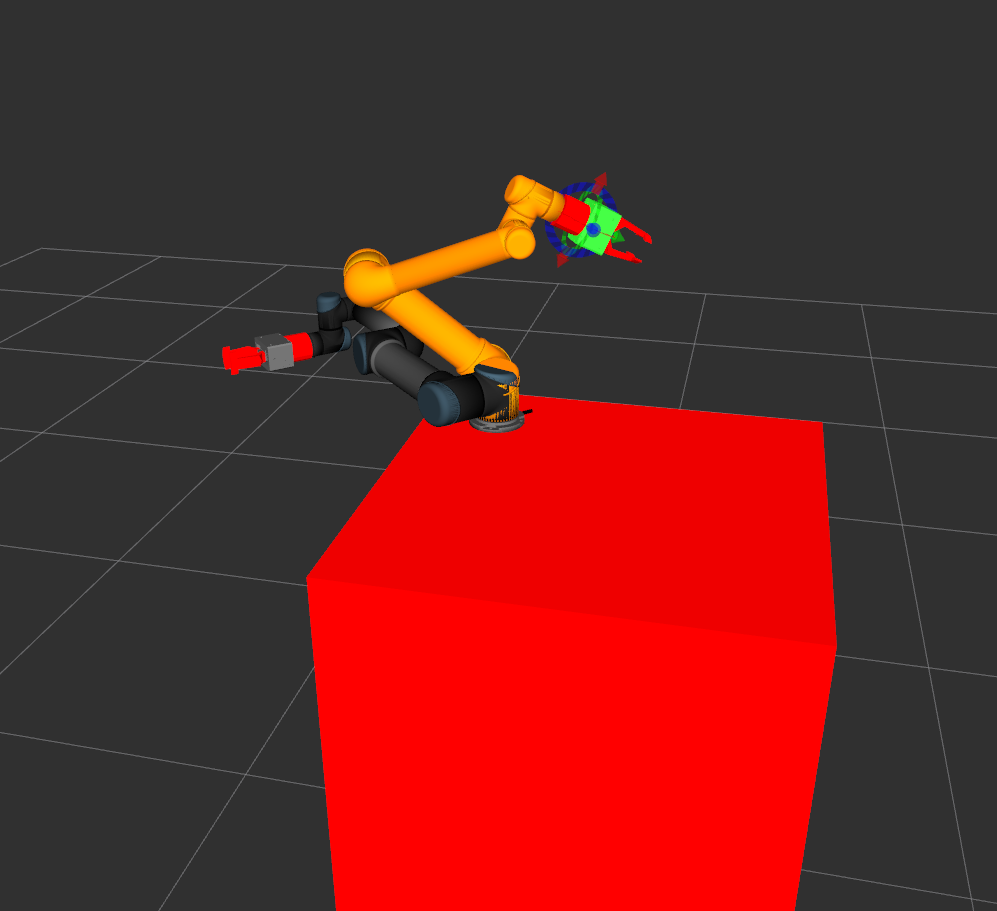
\includegraphics[height=8cm]{images/Modell.png}
	\caption{Das für die Simulation und MoveIt-Bahnplanung verwendete URDF-Modell der statischen Szene.}
	\label{urdfModell}
\end{figure}
